\documentclass[12pt, a4paper, twoside]{article}
\usepackage[utf8]{inputenc}
\usepackage{amsrefs}

% font size could be 10pt (default), 11pt or 12 pt
% paper size coulde be letterpaper (default), legalpaper, executivepaper,
% a4paper, a5paper or b5paper
% side coulde be oneside (default) or twoside 
% columns coulde be onecolumn (default) or twocolumn
% graphics coulde be final (default) or draft 
%
% titlepage coulde be notitlepage (default) or titlepage which 
% makes an extra page for title 
% 
% paper alignment coulde be portrait (default) or landscape 
%
% equations coulde be 
%   default number of the equation on the rigth and equation centered 
%   leqno number on the left and equation centered 
%   fleqn number on the rigth and  equation on the left side
%	
\author{Sven Fiergolla}
\title{Universelle Turingmaschine mit zwei Zuständen/Symbolen}
\date{\today}

\begin{document}
 
\maketitle


\section{Einführung}
\subsection{Informelle Definition der Turingmaschine}
%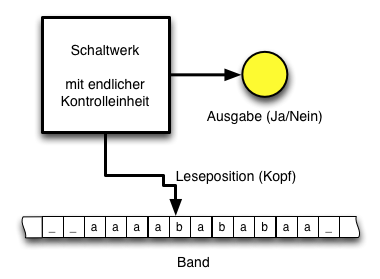
\includegraphics[scale=1]{TMKonzept.png}
Turingmaschinen (im folgenden TM), benannt nach \textit{Alan M. Turing}, sind das allgemeine Modell der theoretischen Informatik.
Sie bestehen aus einem \textit{unendlichen Band}, welches die Eingabe beinhaltet, einem \textit{Lese/Schreibkopf} welcher eine eindeutige Position auf dem Band hat und einem \textit{Steuerungselement}, häufig beschrieben durch eine (partielle) Übergangsfunktion.


\subsection{Formale Definition der Turingmaschine}
Formal definieren wir die Turingmaschine als Septupel $\mathbf{ M = (Q,\Sigma,\Gamma,q_0,\delta,\Square,F)} $
 wobei:

\begin{description}


 \item $\mathbf{ Q = }$ die endliche Zustandsmenge
 \item $\mathbf{ \Sigma = }$ das endliche Eingabealphabet
 \item $\mathbf{ \Gamma = }$ das endliche Bandalphabet und es gilt {\Sigma \subset \Gamma }
 \item $\mathbf{ q_0 = }$ der Anfangszustand
 \item $\mathbf{ \delta = }$die (partielle) Überführungsfunktion
 \item $\mathbf{ \Square = }$steht für das leere Feld (Blank)
 \item $\mathbf{F = }$ die Menge der akzeptierenden Endzustände

\end{description}

 
 


\subsection{universelle Turingmaschinen}
In der obigen Definition ist das Programm fest in die Maschine eingebaut und kann nicht verändert werden. Kodiert man die Beschreibung einer Turingmaschine als hinreichend einfache Zeichenkette, so kann man eine sogenannte universelle Turingmaschine – selbst eine Turingmaschine – konstruieren, welche eine solche Kodierung einer beliebigen Turingmaschine als Teil ihrer Eingabe nimmt und das Verhalten der kodierten Turingmaschine auf der ebenfalls gegebenen Eingabe simuliert. Aus der Existenz einer solchen universellen Turingmaschine folgt zum Beispiel die Unentscheidbarkeit des Halteproblems. Eine ähnliche Idee, bei der das Programm als ein Teil der veränderbaren Eingabedaten betrachtet wird, liegt auch fast allen heutigen Rechnerarchitekturen zugrunde (Von-Neumann-Architektur).

Formal ist eine universelle Turingmaschine eine Maschine {\displaystyle UTM_{\phi }} UTM_{\phi }, die eine Eingabe {\displaystyle w\|x} w\|x liest. Das Wort {\displaystyle w} w ist hierbei eine hinreichend einfache Beschreibung einer Maschine {\displaystyle M_{w}} M_{w}, die zu einer bestimmten Funktion mit Eingabe {\displaystyle x} x die Ausgabe berechnet. {\displaystyle \|} \| ist ein Trennzeichen zwischen Programmbeschreibung und Eingabe. {\displaystyle UTM_{\phi }} UTM_{\phi } simuliert also das Verhalten von {\displaystyle M_{w}} M_{w} mit Hilfe der Funktionsbeschreibung {\displaystyle w} w und der Eingabe {\displaystyle x} x. Der Index {\displaystyle \phi } \phi  in {\displaystyle UTM_{\phi }} UTM_{\phi } zeigt an, dass es nicht nur eine einzige universelle Turingmaschine gibt. So könnten z. B. {\displaystyle UTM_{1}} UTM_{1} und {\displaystyle UTM_{2}} UTM_{2} verschiedene Wörter verstehen. Das Wort {\displaystyle w} w muss dabei in einer Sprache codiert sein, die die {\displaystyle UTM_{\phi }} UTM_{\phi } versteht.





\paragraph{Outline}




\section{Universelle TM mit nur zwei Zuständen}

\section{TM mit einem Zustand niemals universell}

\section{Universelle TM mit zwei Symbolen}

\section{Fazit}




\end{document}
